\begin{figure}
  \centering
    \includegraphics[width=0.5\textwidth]{img/hand.eps}
  \caption{ReFlex Beta Hand}
  \label{fig:hand}
\end{figure}

\begin{figure}
  \centering
    \includegraphics[width=0.5\textwidth]{img/annotated_finger.eps}
  \caption{Close-up of a ReFlex Beta Hand finger}
  \label{fig:finger}
\end{figure}



\subsection{setup}

\subsubsection{Slave system}

In this setup the slave is characterized by a ReFlex Beta (RightHand Robotics) robotic hand. 

This device is made by the Harvard Biorobotics Lab and the Yale Grab Lab, it is a three fingered hand. Each finger is controlled by a single motor that pull the tendon in the finger, this tendon is connected to both the proximal and distal joint. This architecture allows each finger to shape itself to the object shape during the grasp. The fingers are distributed to optimize the object grasping, two finger are positioned on a side and the third is on the opposite one (Figure \ref{fig:hand}). 
During the experiments the hand must remain blocked in the initial position, the back looks downwards and the fingers upwards. 
This hand has a main particularity, on the surface are distributed 38 pressure sensors, for every finger there are 5 sensors on the proximal phalanx and 4 on the distal (Figure \ref{fig:finger}), the rest is on the palm. With this distribution it can do very precise pressure measures. 
The device is controlled by a Ethernet cable connected to a personal computer that handle every communication between the master and the slave system, the producers provide a ROS node to handle it.

\subsubsection{Master system}

The master has a little harder structure, it's mainly composed by a Leap Motion to recognize the user hand movements and a glove to give the feedback.

\textbf{\textit{Leap motion}} is an input device that allow to track the hand and fingers movements, is composed by two infrared (IR) cameras and three infrared leds, with this components it can calculate the distance of every point in his field of vision, from this map it can say if and where the user hands are. 
In \cite{weichert2013analysis} is presented a study of the precision and the stability of leap motion. For the purpose of this experiments the tracking provided by this device is enough accurate.

Instead the "glove" is homemade, it is composed by some \textbf{\textit{vibrating mini-motors}} fixed to the user hand and controlled by an Arduino Mega.

\textbf{\textit{Arduino}} is an open-source electronic prototyping platform that allow to create interactive electronic objects. It can be programmed through the Arduino IDE, that includes a GUI to write sketch (script in Arduino slang), the code compiler and a "programmer" to upload the compiled code on the device. Arduino is connected to the rest of the system through a serial cable.

Each mini-motor is connected to the Arduino through the PWM (Pulse Width Modulation), a signal switched between ON-OFF (5-0V), that returns a value between 0-255 according to the duty-cycle.
The mini-motors need of a simple electronic circuit to be controlled by a PWM signal (Figure \ref{fig:breadboard}).

The minimum number of motors to provide a significative feedback of the robotics hand measures is six, two for everyone of the three fingers. Everyone is wired to the same breadboard and fixed to the hand by a velcro strap.


\begin{figure}
  \centering
    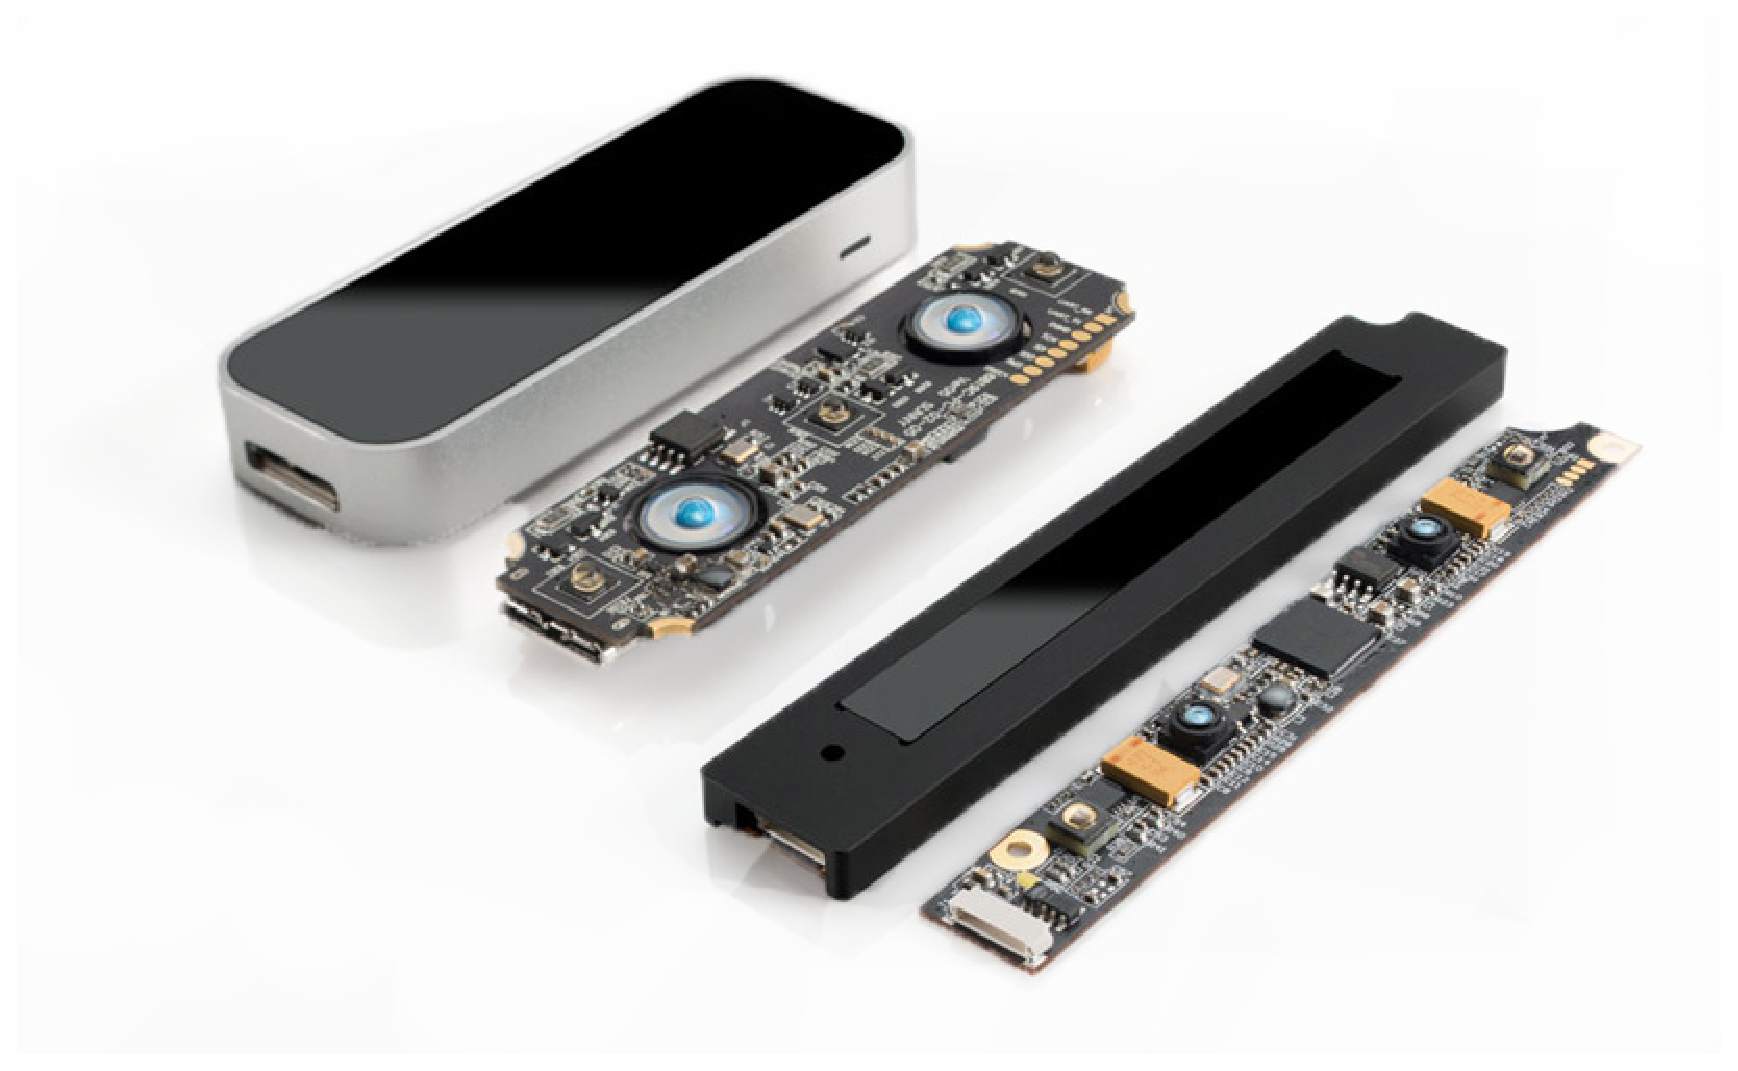
\includegraphics[width=0.5\textwidth]{img/leap_motion.eps}
  \caption{Leap motion}
  \label{fig:leap_motion}
\end{figure}

\begin{figure}
  \centering
    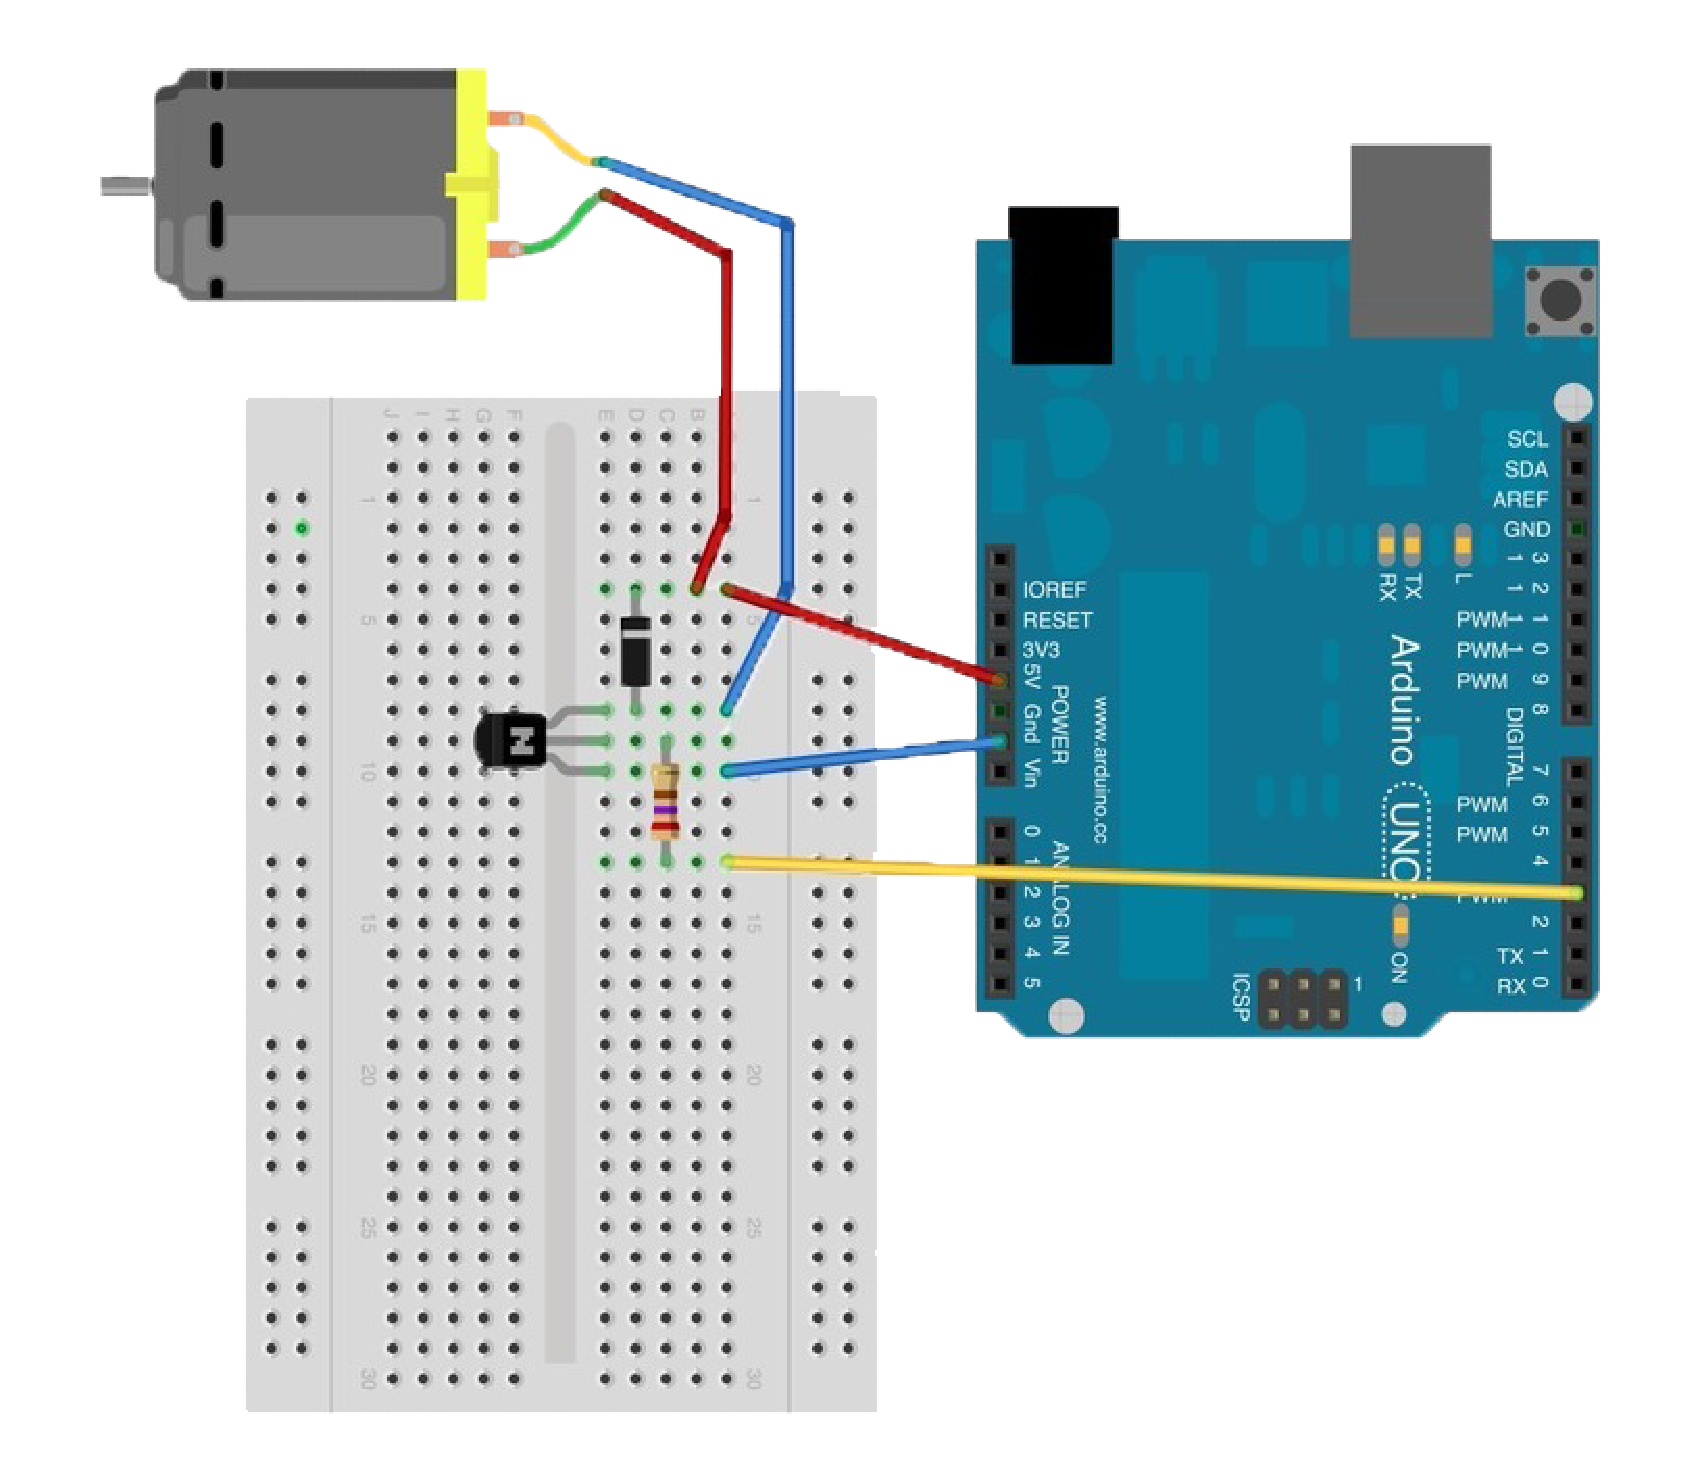
\includegraphics[width=0.5\textwidth]{img/breadboard.eps}
  \caption{Breadboard for vibratory mini-motor}
  \label{fig:breadboard}
\end{figure}

\subsection{Software architecture}

The entire system is handled by \textbf{\textit{ROS (Robot Operating System)}}, a large collection of software frameworks that mainly allows to the system devices to communicate each other. This platform is  characterised by few concepts, the two most important are node and topic. 

A node is a process that performs computation, many nodes communicate each other using topics. This software design method provides several benefits, 
The developer designs the software in a easier in comparison to monolithic systems, every crash is isolated to the interested node, node implementation is hidden because each node exposes only a minimal API to the others.

The ROS structure of the system is shown by the block diagram in figure \ref{fig:rosstructure} where the ovals are the nodes and the rectangles are the topics. 
The graph represents perfectly the system flow from the leap motion camera to the arduino that handles the vibratory glove.

\par

\textit{leap\textunderscore motion\textunderscore skeleton} is the node of rosleapmotion package that publish the a message with the information of every hand segment perceived by the leap motion, this messages contain a vector with the translation and a quaternion with the orientation.

\textit{tf\textunderscore to\textunderscore CommandHand} is a node with the purpose to filters the tf messages discarding those are not needed and convert the orientation matrix from quaternion to axis-angle notation. With this two simple operation we can isolate the rotation angle of the interesting finger phalanges. Then these angles are published on the reflex\textunderscore commander topic.

\textit{reflex\textunderscore move}





\begin{figure}
  \centering
    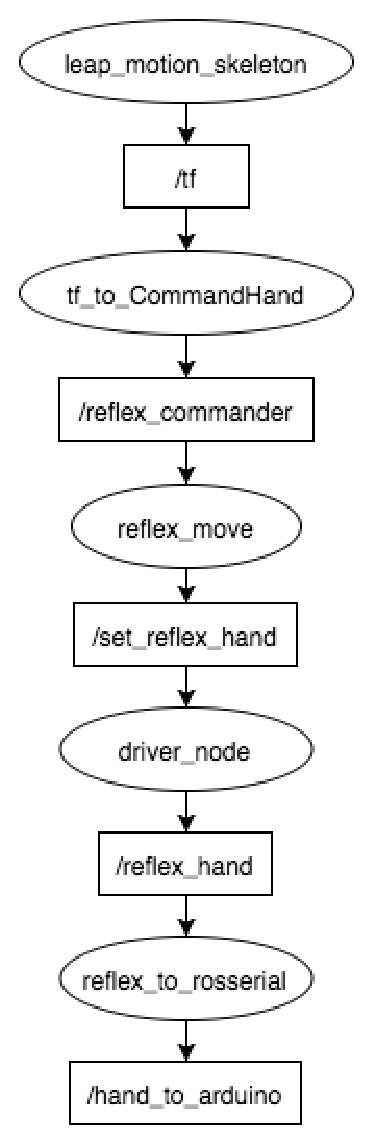
\includegraphics[width=0.3\textwidth]{img/ROS_structure.eps}
  \caption{ROS architecture}
  \label{fig:rosstructure}
\end{figure}
